%\documentclass{article}
%\usepackage{graphicx,subfigure}
%\begin{document}

\begin{figure}[!h]
  \centering
  \subfigure[Relevant to Figure~\ref{fig:twist}] {
  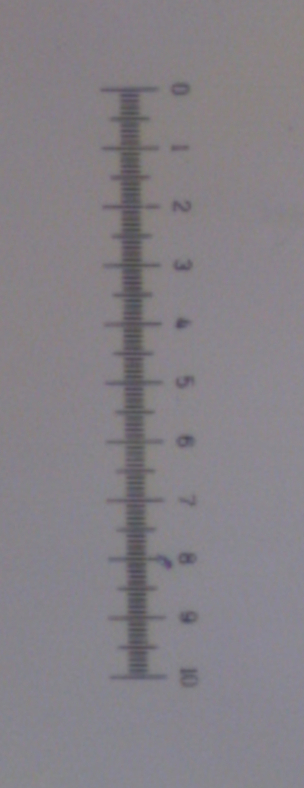
\includegraphics[scale=0.55,angle=90]{mic25x2592x1944rotcrop.jpg}
  }\vfill
  \subfigure[Relevant to Figure~\ref{fig:notwist}] {
  
\includegraphics[scale=0.55]{mic25x2592x1944crop.jpg}
  }\vfill
  \subfigure[Relevant to Figure~\ref{skin:hs}]{
  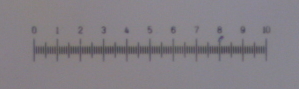
\includegraphics[scale=0.33]{figgradslide25xcrop.png}
  }\vfill
  \subfigure[Relevant to Figure~\ref{fig:fibre3types}] {
  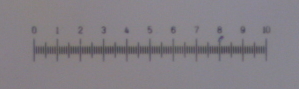
\includegraphics[scale=0.38]{figgradslide25xcrop.png}
  }

% 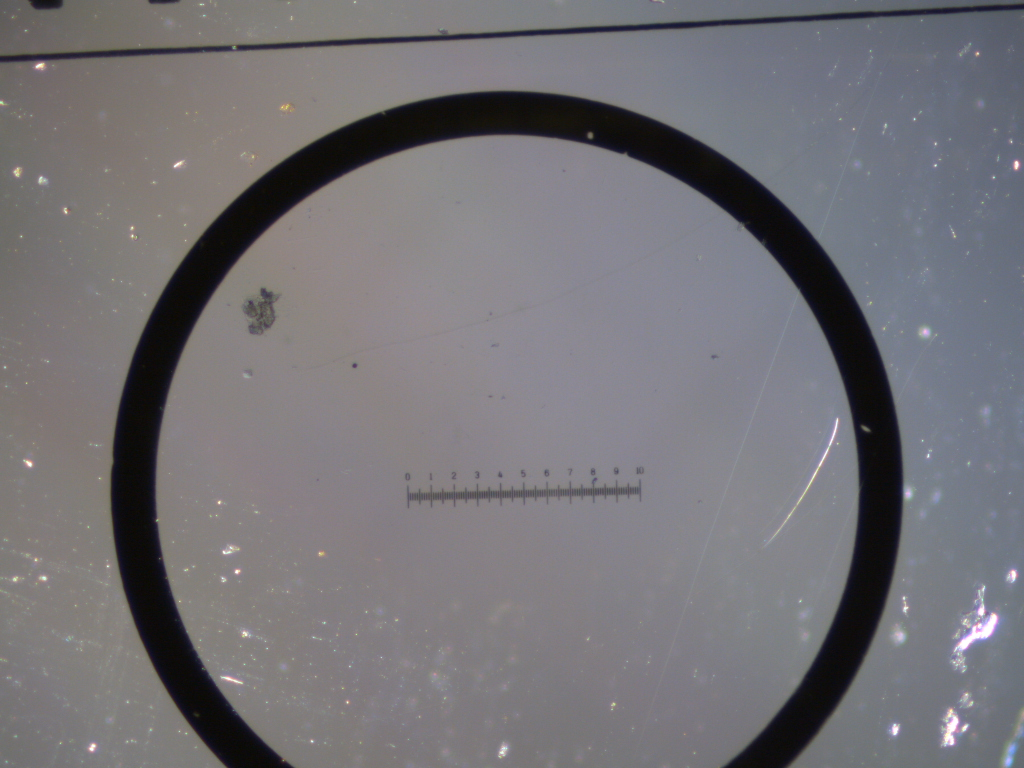
\includegraphics[scale=0.33]{figgradslide25x.png}
% 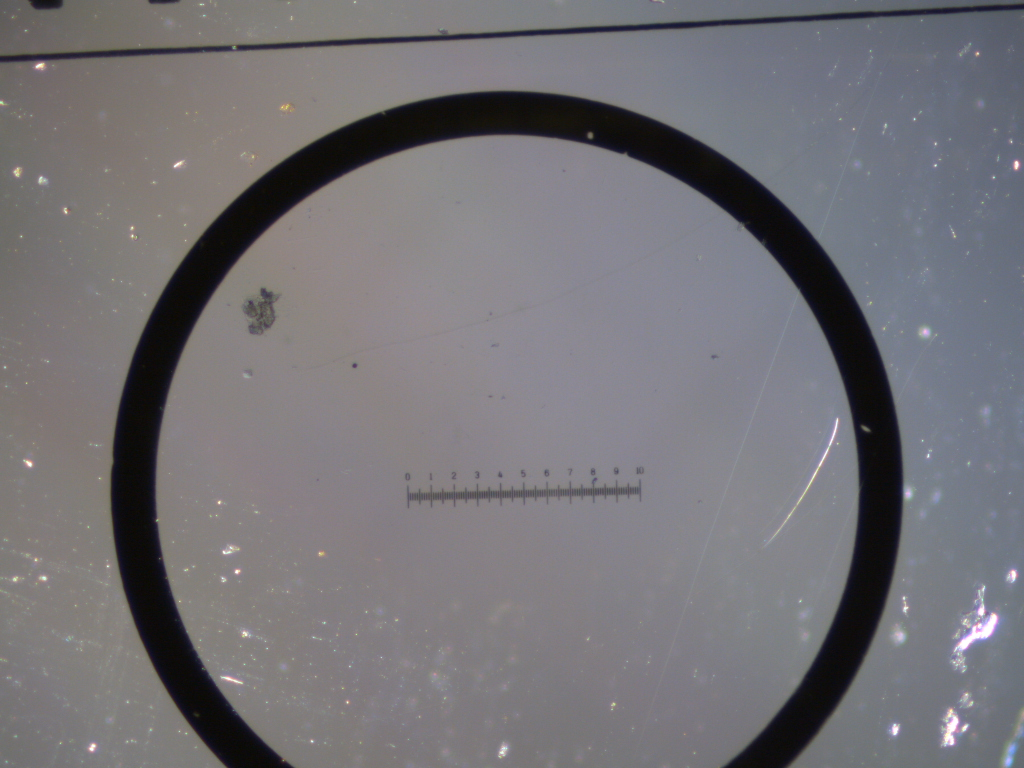
\includegraphics[scale=1.0]{figgradslide25x.png}

  \caption{Photomicrographs of a graduated slide at 25x microscope magnification, at various scale factors and resolutions, to match those of each of the text Figures indicated in the subcaptions.}
  \label{fig:gradslide25x}
\end{figure}

%\end{document}

